\section{Tournament Manager Software}\label{secTournamentManagerSoftware}

Tournament Manager\footnote{\url{http://github.com/davechurchill/StarcraftAITournamentManager}} is an open-source software created by the organizers of the AIIDE Starcraft AI Competition. It is also used in remaining two competitions to some extent. 

It uses a server-client architecture with one machine acting as a server (coordinating the matchups and processing results) and any number of other machines acting as clients (running the bots and StarCraft). The tournament manager is written entirely in Java, and can be run on Windows 7 or higher, either on a physical machine or a virtual machine. All data sent and received is compressed and passed through Java sockets, so no special network configuration is required to run the software.

\subsection{Server}

When running the software, one machine acts as a server for the tournament. The server is a central repository where all bot files (including file I/O) data, cumulative results, and replay files are stored. The server also monitors each client remotely and outputs results data in HTML format. Tournament status can be viewed in real time via the server GUI (see Figure~\ref{tmServerGUI}). 

\begin{figure}[h]
  \centering
  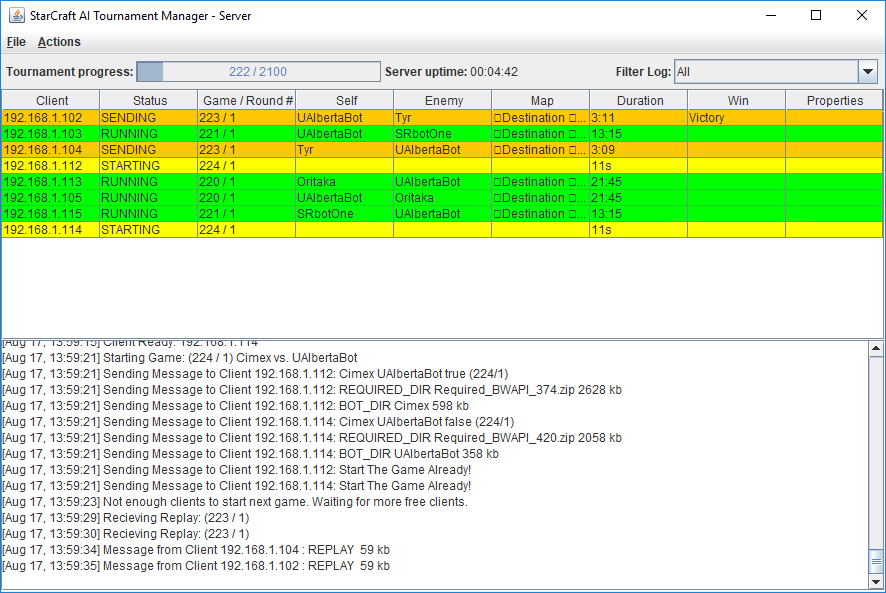
\includegraphics[width=1\columnwidth]{fig/tournament-manager-screenshot.png}
  \caption{Tournament Manager Server GUI}
  \label{tmServerGUI}
\end{figure}

The server program has a threaded component which monitors for new client connections and detects client disconnections, maintaining a current list of clients which can have one of the following statuses:

\begin{itemize}
\item READY: Client is free and ready to start a game of StarCraft
\item STARTING: Client has started the StarCraft LAN lobby but the match has not yet begun
\item RUNNING: Client is currently running a game of StarCraft
\item SENDING: Client has finished the game and is sending results and data back to the server.
\end{itemize}

The server's main scheduling loop tries to schedule the next game from the games list every 2 seconds. Normally a new game can be started only if both of these conditions are true:

\begin{enumerate}
\item two or more Clients are READY, and
\item no clients are STARTING.
\end{enumerate}

\noindent Once these two conditions are met, the server sends the required bot files, map files, BWAPI version, and DLL injector to the client machines, specifying one client as the host and one as the away machine. The status of those clients is then set to STARTING.

Each client is handled by a separate thread in the server, and if the client is STARTING, RUNNING, or SENDING, it sends periodic status updates back to the server for remote monitoring. Periodic data updates are sent to the server once per second and include current game time, time-out information, map, game ID, etc. When a client finishes a game it also sends the results, I/O data files and replay files, which are all stored on the server. This process is repeated until the tournament has finished.

Shutting down the server via the GUI will cause all the client games to stop and all clients to shut down and properly clean up remote machines. The tournament can be resumed upon re-launching the server as long as the results file, games list, and settings file do not change. If the server is shut down with games in progress (results not yet received by the server), those games will be rescheduled and played again.

\subsection{Client}

The client software can be run on as many machines as needed. After an initial setup of the client machine (installing StarCraft, etc.) the client software connects to the server machine via LAN and awaits instructions.

The client machine will stay idle until it receives instructions from the server that a game should be run. Once the client receives the instructions and required files from the server, it ensures that no current StarCraft processes are running, records a current list of the running processes on the client machine, writes the BWAPI settings file, and starts the game. When the game starts, a custom BWAPI Tournament Module is injected which outputs a GameState file to disk every few frames -- this monitors the current state of the StarCraft game in progress. The client software reads this file to check for various conditions such as bot time-outs, crashes, no game frame progression, and game termination. While the game is running, the client also sends the contents of the GameState file to the server once per second for centralized monitoring.

Once the game has ended, or was terminated for any reason, the results of the game, replay files, and file I/O data are sent to the server. After this, the client shuts down any processes on the machine which were not running when the game began, to prevent things like crashed proxy bots or stray threads from hogging system resources from future games. StarCraft is shut down, the machine is cleaned of any files written during the previous game, and the client status is reported back to the server as READY.




